\documentclass{standalone}
\usepackage{tikz}
\usetikzlibrary{matrix}

\begin{document}
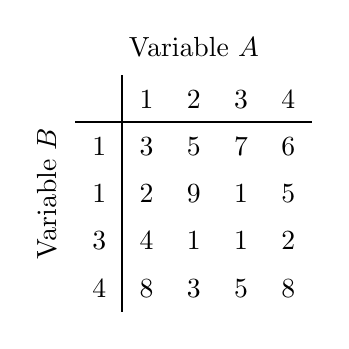
\begin{tikzpicture}
  \matrix[
    matrix of nodes,
    nodes = {
      anchor = center, 
      minimum size = .6cm
    }
  ] (tab) at (0,0) {
     &  1  &  2  &  3  &  4  \\
  1  &  3  &  5  &  7  &  6  \\ 
  1  &  2  &  9  &  1  &  5  \\
  3  &  4  &  1  &  1  &  2  \\
  4  &  8  &  3  &  5  &  8  \\
};

  % The two row/column lines
  \draw[thick] (tab-2-1.north west) -- (tab-2-5.north east);
  \draw[thick] (tab-1-2.north west) -- (tab-5-2.south west);
 
  % The two labels
  \node[anchor = south]              at (tab.north) {Variable $A$}; 
  \node[anchor = south, rotate = 90] at (tab.west)  {Variable $B$}; 
\end{tikzpicture}
\end{document}
